\section{Organisation}
\subsection{Les outils utilisés}

Afin de nous coordonner et de gérer les versions, nous avons utilisé git. Le dépôt est accessible à l'adresse \url{https://github.com/Neressea/MovieManager}. \\
Pour générer l'UML et simplifier le lancement des tests unitaires, nous avons utilisé l'IDE Eclipse. \\
Nous pouvons aussi noter l'utilisation de jar externes pour le JDatePicker qui sert à la sélection de la date et pour les tests unitaires.

\subsection{UML du modèle}

L'UML du modèle a été généré à l'aide du module ObjectAid UML d'Eclipse. \\


\begin{figure}[!ht]
    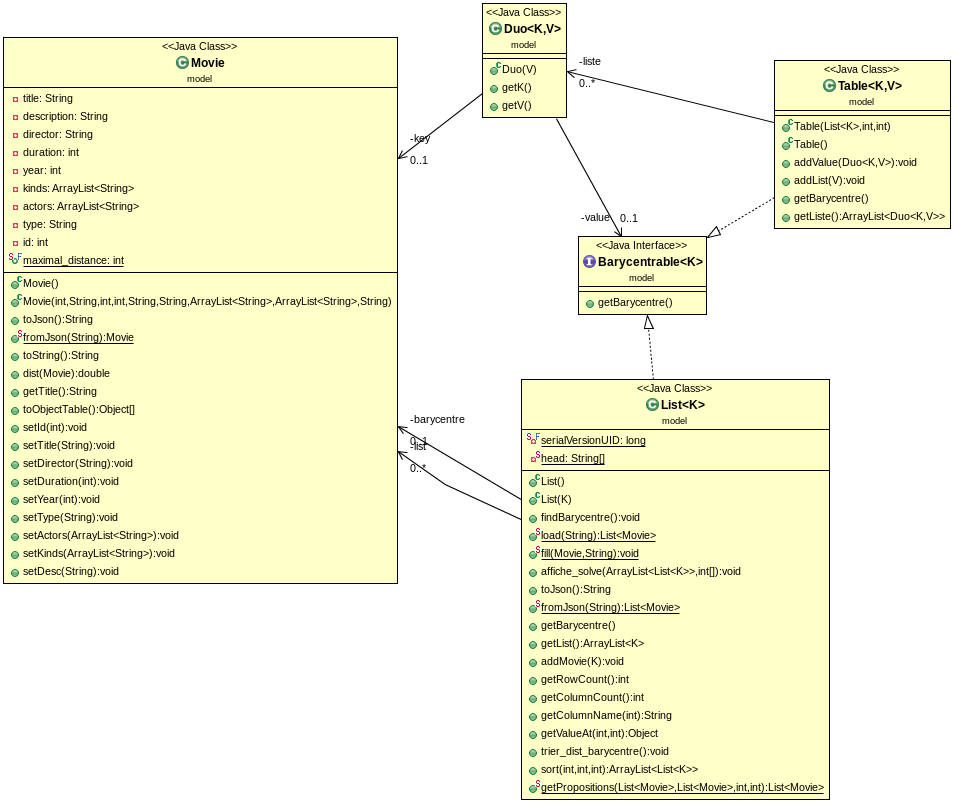
\includegraphics[width=1\textwidth]{./images/uml.png}
    \caption{UML du projet}
\end{figure}

On peut remarquer que l'on a créé une interface Barycentrable qui nous permet de limiter l'utilisation de Duo aux objets en héritant.
Grâce à cela, nous pouvons appeler la méthode getBarycentre() à tout instant.

